\documentclass[10pt,a4paper]{article}

\usepackage{amsmath}
\usepackage{amsfonts}
\usepackage{amssymb}
\usepackage{amsthm}
\usepackage{enumerate}
\usepackage{tikz}

%\theoremstyle{definition}
\newtheorem{theorem}{Theorem}[section]
\newtheorem{prop}[theorem]{Proposition}
\newtheorem{cor}[theorem]{Corollary}
\newtheorem{lemma}[theorem]{Lemma}
\newtheorem{example}[theorem]{Example}
\newtheorem{definition}[theorem]{Definition}

\author{Mitchell Riley}
\title{Root Systems}

\begin{document}
\maketitle

Associated with every semisimple Lie algebra is a structure known as a root system, which efficiently captures many of the features of the Lie algebra. From root systems we can pass through to the Dynkin diagram of a Lie algebra, and by classifying these Dynkin diagrams we can classify all simple Lie algebras.

The precise connection between Lie algebras and root systems is the topic of a future talk. This talk will mainly focus on root systems and Dynkin diagrams in isolation, but we can motivate their definition here.

Let $\mathfrak{g}$ be a semisimple Lie algebra, and $\mathfrak{h}$ a Cartan subalgebra of $\mathfrak{g}$. As we have seen, we can decompose the adjoint representation of $\mathfrak{g}$ as:
\begin{align*}
	\mathfrak{g} = \mathfrak{h} \oplus \left(\bigoplus \mathfrak{g}_\alpha \right)
\end{align*}
where the $\mathfrak{g}_\alpha$ are the subspaces of $\mathfrak{g}$ with `eigenvalue' $\alpha \in \mathfrak{h}^*$. In other words, for any $H \in \mathfrak{h}$ and $X \in \mathfrak{g}_\alpha$
\begin{align*}
	\text{ad}(H)(X) = \alpha(H) \cdot X
\end{align*}

The set of these eigenvalues forms a root system within $\mathfrak{h}^*$.

\section{Root Systems}

\begin{definition}[Root system]

A finite subset $R$ of a Euclidean space $V$ is a root system if:

\begin{enumerate}
\item $R$ spans $V$ and does not contain 0.
\item For any $\alpha \in R$, $-\alpha$ is also a root and these are the only roots proportional to $\alpha$. ($R$ is `reduced')
\item For any $\alpha \in R$, the reflection $W_\alpha$ in the hyperplane $\alpha^\bot$ maps $R$ to itself.
\item For each $\alpha, \beta \in R$, $W_\alpha(\beta) - \beta$ is an integer multiple of $\alpha$.
\end{enumerate}
\end{definition}

Reflecting a vector $\beta$ through a hyperplane with normal $\alpha$ can be thought of as subtracting from $\beta$ twice the projection of $\beta$ onto $\alpha$. Therefore, the reflections $W_\alpha$ can be written as:
\begin{align*}
	W_\alpha(\beta) = \beta - 2 \frac{(\beta, \alpha)}{(\alpha, \alpha)} \alpha
\end{align*}

From this, it is clear that point 4) is equivalent to requiring that
\begin{align*}
	n_{\beta \alpha} = 2 \frac{(\beta, \alpha)}{(\alpha, \alpha)}
\end{align*}
is an integer.

This condition puts strong restrictions on the angle between two roots. Let $\theta$ be the angle between the roots $\alpha$ and $\beta$. Then:

\begin{align*}
	n_{\beta \alpha} = 2 \frac{(\beta, \alpha)}{(\alpha, \alpha)} &= 2 \cos{\theta} \frac{\|\beta \|}{\| \alpha \|} \\
	n_{\beta \alpha} n_{\alpha \beta} &= (2 \cos \theta)^2
\end{align*}
This must be an integer. Because $2 \cos \theta \in [-2, 2]$, the only possible values for $\cos \theta$ are 0, $\pm \frac{1}{2}$, $\pm \frac{\sqrt{2}}{2}$, $\pm \frac{\sqrt{3}}{2}$ and $\pm \frac{\sqrt{4}}{2} = \pm 1$, corresponding to angles of $\pi/2$, $\pi/3$ or $2 \pi/3$, $\pi/4$ or $3 \pi/4$, $\pi/6$ or $5 \pi/6$, $0$ or $\pi$.

\begin{example}
We can now easily classify root systems of rank 1 and 2. For rank 1, because of condition 2) there is only one possibility, $A_1$. For systems of rank 2, condition 3) means that the angles between adjacent roots must be equal. All of the options $\frac{\pi}{2}$, $\frac{\pi}{3}$, $\frac{\pi}{4}$ and $\frac{\pi}{6}$ occur, as $A_1 \times A_1$, $A_2$, $B_2$ and $G_2$. Note that $A_1 \times A_1$ is the orthogonal direct sum of two root systems. Root systems that are not such a sum are \emph{irreducible}. In the other 3 cases, the relative lengths of the roots are fixed by condition 4).
\end{example}

\begin{definition}
Let $R$ be a root system in a vector space $V$. The Weyl group of $R$ is the subgroup $W$ of $GL(V)$ generated by the symmetries $W_\alpha$, $\alpha \in R$.
\end{definition}

Every Weyl group is a Coxeter group, but not every Coxeter group is
the Weyl group of some root system.

\begin{example}
In the root systems above, the Weyl group is isomorphic to the dihedral group of order $2n$, with $n=2$, $n=3$, $n=4$ and $n=6$ respectively.
\end{example}

\section{Simple Roots}

Let $\alpha, \beta$ be two roots with $\beta \neq \pm \alpha$. The $\alpha$-string through $\beta$ is all roots of the form
\begin{align*}
	\beta - p \alpha, \beta - (p - 1) \alpha, \dots, \beta - \alpha, \beta, \beta + \alpha, \beta + 2 \alpha, \dots, \beta + q \alpha
\end{align*}

\begin{prop}
The $\alpha$-string through $\beta$ is at most four roots long, i.e., $p + q \leq 3$.
\end{prop}
\begin{proof}
First note that $W_\alpha(\beta + q \alpha) = \beta - p \alpha$, as the reflection must take one end of the string to the other. But also,
\begin{align*}
	W_\alpha(\beta + q \alpha) = (\beta - n_{\beta \alpha} \alpha) - q \alpha
\end{align*}

Equating the two sides we have $p - q = n_{\beta \alpha}$. Now consider the same string shifted to start at $\beta - p \alpha$. Then $p' = 0$ and $q' = -n_{\beta \alpha}$ which must be an integer less than 4.

Therefore the chain is at most four roots long.
\end{proof}

\begin{cor}
Let $\alpha, \beta$ be two roots with $\beta \neq \pm \alpha$. Then
\begin{align*}
	(\beta, \alpha) > 0 \Rightarrow \alpha - \beta \text{ is a root} \\
	(\beta, \alpha) < 0 \Rightarrow \alpha + \beta \text{ is a root} \\
\end{align*}
If $(\beta, \alpha) = 0$, then $\alpha - \beta$ and $\alpha + \beta$ are either both roots or neither roots.
\end{cor}
These are not hard to show; for example, if $(\beta, \alpha) > 0$, then $n_{\beta \alpha} > 0$ and $p > q$, so $p \neq 0$.

Complete information about a root system can be recovered from particular subsets of the roots. Choose a direction $l$, and let $R = R^+ \cup R^-$ be the disjoint union of positive and negative roots. A positive root is then \emph{simple} if it is not the sum of two other positive roots.

\begin{prop}
If $\alpha$ and $\beta$ are distinct simple roots, then neither $\alpha - \beta$ nor $\beta - \alpha$ are roots.
\end{prop}
\begin{proof}
$\alpha = \beta + (\alpha - \beta)$, so $\alpha - \beta$ cannot be in $R^+$, otherwise $\alpha$ would not be simple. Similarly, $\beta - \alpha = -(\alpha - \beta)$ cannot be in $R^+$. So neither can be a root.
\end{proof}

\begin{cor}
If $\alpha$ and $\beta$ are distinct simple roots, then $(\beta, \alpha) \leq 0$, i.e., the angle between distinct simple roots cannot be obtuse.
\end{cor}
\begin{cor}
The simple roots are linearly independent.
\end{cor}

This follows from the fact that if a set of vectors lies on one side of a hyperplane, with all mutual angles at least $\frac{\pi}{2}$, then they must be linearly independent. Proof is left as an exercise!

\begin{cor}
There are exactly $n$ simple roots, where $n$ is the rank of the root system.
\end{cor}

Because the simple roots are linearly independent, it is clear that the number of simple roots cannot exceed the rank of the root system.

\section{Dynkin Diagrams}

The Dynkin diagram of a root system is a graph with one vertex for each simple root, where two simple roots are connected in a way depending on the angle $\theta$ between them:

\begin{tabular} { c l }
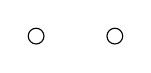
\begin{tikzpicture}
	\draw[fill=white] (0,0) circle(.1);
	\draw[fill=white] (1,0) circle(.1);
\end{tikzpicture}
& if $\theta = \pi / 2$ \\

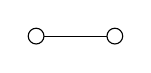
\begin{tikzpicture}
	\draw (0,0) -- (1,0);

	\draw[fill=white] (0,0) circle(.1);
	\draw[fill=white] (1,0) circle(.1);
\end{tikzpicture}
& if $\theta = 2 \pi / 3$ \\

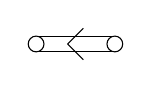
\begin{tikzpicture}
	\draw (0,.1) -- (1,.1);
	\draw (0,-.1) -- (1,-.1);
	\draw (.4,0) -- (.6,0.2);
	\draw (.4,0) -- (.6,-0.2);

	\draw[fill=white] (0,0) circle(.1);
	\draw[fill=white] (1,0) circle(.1);
\end{tikzpicture}
& if $\theta = 3 \pi / 4$ \\

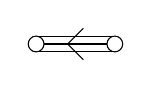
\begin{tikzpicture}

	\draw (0,0) -- (1,0);
	\draw (0,.1) -- (1,.1);
	\draw (0,-.1) -- (1,-.1);
	\draw (.4,0) -- (.6,0.2);
	\draw (.4,0) -- (.6,-0.2);

	\draw[fill=white] (0,0) circle(.1);
	\draw[fill=white] (1,0) circle(.1);
\end{tikzpicture}
& if $\theta = 5 \pi / 6$ \\
\end{tabular}

When there is a single line, both roots are the same length. If there are two or three lines between roots, the arrow points from the longer root to the shorter root.

\begin{theorem}
A root system is irreducible if and only if its Dynkin diagram is connected.
\end{theorem}
\begin{proof}
If $R$ is the sum of two subsystems $R_1$ and $R_2$, then we can let the union of the two sets of simple roots $S_1$ and $S_2$ be the set of simple roots for $R$. Take any $\alpha \in S_1$ and $\beta \in S_2$. These are orthogonal, so cannot be connected in the Dynkin diagram of $R$. It follows that the Dynkin diagram of $R$ cannot be connected.

Conversely, if the Dynkin diagram is not connected, then the set of simple roots has a nontrivial partition $S = S_1 \cup S_2$ such that every root in $S_1$ is orthogonal to those in $S_2$. The vector spaces spanned by $S_1$ and $S_2$ are therefore orthogonal, and $R$ is the orthogonal sum of $R_1$ and $R_2$.
\end{proof}

We now come to the main classification theorem for root systems, which as we see later will exactly correspond to the classification of simple Lie algebras. This classification also helps us explain some of the interesting isomorphisms between Lie algebras of small dimension.

\begin{theorem}
They Dynkin diagrams of irreducible root systems are precisely:

\begin{tikzpicture}
	\fill[color=white] (0,0) circle(.1);
\end{tikzpicture}

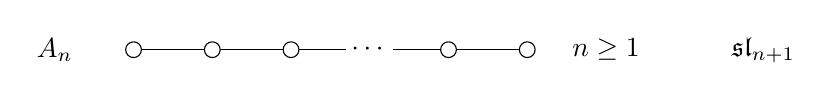
\begin{tikzpicture}

	\draw (0,0) -- (1,0);
         \draw (2,0) -- (2.7,0);
         \draw (1,0) -- (2,0);
	\draw (3.3, 0) -- (4,0);
	\draw (4,0) -- (5,0);

	\draw[fill=white] (0,0) circle(.1);
	\draw[fill=white] (1,0) circle(.1);
	\draw[fill=white] (2,0) circle(.1);
	\draw[fill=white] (4,0) circle(.1);
	\draw[fill=white] (5,0) circle(.1);

	\node at (3,0) {$\cdots$};
	\node at (-1,0) {$A_{n}$};
	\node at (6,0)  {$n \geq 1$};
	\node at (8,0)  {$\mathfrak{sl}_{n+1}$};
\end{tikzpicture}

\vspace*{0.3cm}

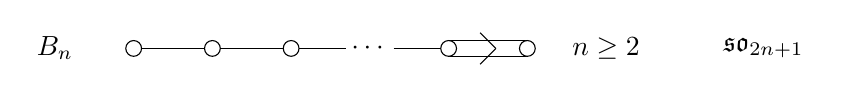
\begin{tikzpicture}

	\draw (0,0) -- (2.7,0);
	\draw (3.3, 0) -- (4,0);
	\draw (4,0.1) -- (5,0.1);
	\draw (4,-0.1) -- (5,-0.1);
	\draw (4.4,0.2) -- (4.6,0);
	\draw (4.4,-0.2) -- (4.6,0);

	\draw[fill=white] (0,0) circle(.1);
	\draw[fill=white] (1,0) circle(.1);
	\draw[fill=white] (2,0) circle(.1);
	\draw[fill=white] (4,0) circle(.1);
	\draw[fill=white] (5,0) circle(.1);

	\node at (3,0) {$\cdots$};
	\node at (-1,0) {$B_{n}$};
	\node at (6,0)  {$n \geq 2$};
	\node at (8,0)  {$\mathfrak{so}_{2n+1}$};
\end{tikzpicture}

\vspace*{0.3cm}

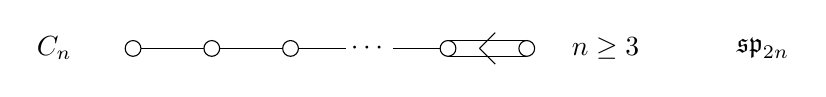
\begin{tikzpicture}

	\draw (0,0) -- (2.7,0);
	\draw (3.3, 0) -- (4,0);
	\draw (4,0.1) -- (5,0.1);
	\draw (4,-0.1) -- (5,-0.1);
	\draw (4.4,0) -- (4.6,0.2);
	\draw (4.4,0) -- (4.6,-0.2);

	\draw[fill=white] (0,0) circle(.1);
	\draw[fill=white] (1,0) circle(.1);
	\draw[fill=white] (2,0) circle(.1);
	\draw[fill=white] (4,0) circle(.1);
	\draw[fill=white] (5,0) circle(.1);

	\node at (3,0) {$\cdots$};
	\node at (-1,0) {$C_{n}$};
	\node at (6,0)  {$n \geq 3$};
	\node at (8,0)  {$\mathfrak{sp}_{2n}$};
\end{tikzpicture}

\vspace*{0.3cm}

\begin{tikzpicture}

	\draw (0,0) -- (2.7,0);
	\draw (3.3, 0) -- (4,0);
	\draw (4,0) -- (5,-.5);
	\draw (4,0) -- (5,.5);

	\draw[fill=white] (0,0) circle(.1);
	\draw[fill=white] (1,0) circle(.1);
	\draw[fill=white] (2,0) circle(.1);
	\draw[fill=white] (4,0) circle(.1);
	\draw[fill=white] (5,-.5) circle(.1);
	\draw[fill=white] (5,.5) circle(.1);

	\node at (3,0) {$\cdots$};
	\node at (-1,0) {$D_{n}$};
	\node at (6,0)  {$n \geq 4$};
	\node at (8,0)  {$\mathfrak{so}_{2n}$};
\end{tikzpicture}

\begin{tikzpicture}

	\draw (0,0) -- (4,0);
	\draw (2,0) -- (2,1);

	\draw[fill=white] (0,0) circle(.1);
	\draw[fill=white] (1,0) circle(.1);
	\draw[fill=white] (2,0) circle(.1);
	\draw[fill=white] (2,1) circle(.1);
	\draw[fill=white] (3,0) circle(.1);
	\draw[fill=white] (4,0) circle(.1);

	\node at (-1,0) {$E_6$};

\end{tikzpicture}

\begin{tikzpicture}

	\draw (0,0) -- (5,0);
	\draw (2,0) -- (2,1);

	\draw[fill=white] (0,0) circle(.1);
	\draw[fill=white] (1,0) circle(.1);
	\draw[fill=white] (2,0) circle(.1);
	\draw[fill=white] (2,1) circle(.1);
	\draw[fill=white] (3,0) circle(.1);
	\draw[fill=white] (4,0) circle(.1);
	\draw[fill=white] (5,0) circle(.1);

	\node at (-1,0) {$E_7$};

\end{tikzpicture}

\begin{tikzpicture}

	\draw (0,0) -- (6,0);
	\draw (2,0) -- (2,1);

	\draw[fill=white] (0,0) circle(.1);
	\draw[fill=white] (1,0) circle(.1);
	\draw[fill=white] (2,0) circle(.1);
	\draw[fill=white] (2,1) circle(.1);
	\draw[fill=white] (3,0) circle(.1);
	\draw[fill=white] (4,0) circle(.1);
	\draw[fill=white] (5,0) circle(.1);
	\draw[fill=white] (6,0) circle(.1);

	\node at (-1,0) {$E_8$};

\end{tikzpicture}

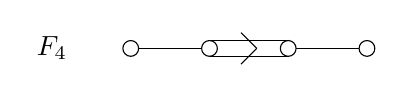
\begin{tikzpicture}

	\draw (0,0) -- (1,0);
	\draw (1,.1) -- (2,.1);
	\draw (1,-.1) -- (2,-.1);
	\draw(2,0) -- (3,0);
	\draw (1.4,0.2) -- (1.6,0);
	\draw (1.4,-0.2) -- (1.6,0);

	\draw[fill=white] (0,0) circle(.1);
	\draw[fill=white] (1,0) circle(.1);
	\draw[fill=white] (2,0) circle(.1);
	\draw[fill=white] (3,0) circle(.1);

	\node at (-1,0) {$F_4$};

\end{tikzpicture}

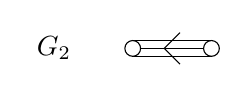
\begin{tikzpicture}

	\draw (0,0) -- (1,0);
	\draw (0,.1) -- (1,.1);
	\draw (0,-.1) -- (1,-.1);
	\draw (.4,0) -- (.6,0.2);
	\draw (.4,0) -- (.6,-0.2);

	\draw[fill=white] (0,0) circle(.1);
	\draw[fill=white] (1,0) circle(.1);

	\node at (-1,0) {$G_2$};

\end{tikzpicture}

\end{theorem}
\begin{proof}
The proof is long but we can sketch the steps involved.

The first step is to note that the angles between roots is all that is required to determine the possible diagrams, i.e., we can ignore any arrows on the edges. Such diagrams are called Coxeter graphs.

A Coxeter graph with $n$ nodes is `admissible' if there are $n$
independent unit vectors in a Euclidean space with the angle between
$e_i$ and $e_j$ being $\pi/2$, $2 \pi/3$, $3 \pi/4$ or $5 \pi/6$ according to the number of lines between $e_i$ and $e_j$ being 0, 1, 2 or 3.

The proof goes as follows:

\begin{enumerate}
\item Any subdiagram of an admissible diagram must also be admissible.
\item An admissible diagram has no cycles.
\item No node has more than three lines to it.
\item In any admissible diagram, any string of nodes connected to each
  other by one line can be collapsed to one node, and the resulting
  diagram remains admissible.
\item Other than $F_4$, a double line must appear on the edge of a
  diagram.
\item Triple nodes with longer legs are inadmissible.
\end{enumerate}

\end{proof}

\end{document}
